\documentclass{template/priloha}

\usepackage{subcaption} 
\usepackage{amsmath} 
\usepackage{enumitem} 
\usepackage{hyperref} % reference
\usepackage{gensymb} % balíček symbolů
\usepackage{booktabs}

\usepackage[toc,page]{appendix}
\usepackage{color} % balíček pro obarvování textů
\usepackage{xcolor}  % zapne možnost používání barev, mj. pro \definecolor
\definecolor{mygreen}{RGB}{0,150,0} % nastavení barev odkazů 
\definecolor{myblue}{RGB}{0,0,200} % nastavení barev odkazů 

\usepackage{listings} % balíček pro formátování zdrojových kódů 
\usepackage[author=,status=final]{fixme} % vkládání poznámek  
% dva módy (status): draft (poznámky se zobrazují v PDF) / final (poznámky se nezobrazují v PDF)
\usepackage{multirow}
\usepackage{hyperref} % pro vkládání odkazu

\usepackage{wrapfig}
\usepackage{epsfig}

\usepackage{blindtext}
\usepackage[T1]{fontenc}
\usepackage[utf8]{inputenc}
\usepackage[czech]{babel}
\usepackage{caption}
\usepackage{biblatex}
\usepackage{graphicx}
\usepackage{fancyhdr}
%\usepackage[backend=biber, style=iso-numeric,sorting=ynt]{biblatex}

\hypersetup{colorlinks=true, linkcolor=myblue, urlcolor=mygreen, citecolor=blue, anchorcolor = magenta,
	 linktocpage = true, frenchlinks } % nastavení barvy odkazů 


\lstset { %
    language=C++,
    backgroundcolor=\color{black!5}, % set backgroundcolor
    basicstyle=\footnotesize  % basic font setting
}

\newcommand{\obr}[1]{[obr. \ref{#1}/str. \pageref{#1}]}
\newcommand{\chapterm}[1]{
    
    \chapter{#1}

    \vspace{-10mm}
}

\addbibresource{kapitoly/text_mecha.bib} % soubor s bibliografií
\nocite{*}

\titlecz{Mechanický BlackBox} % český název práce
\titleen{Mechanical BlackBox} % anglický název práce
\originaltitlecz{BlackBox}
\author{Tomáš Vavrinec} % jméno a příjmení autora
\field{10} % obor (pouze číslo, zbytek vysází šablona - číslo oboru viz http://www.soc.cz/obory-soc/)
\school{Střední průmyslová škola a~Vyšší odborná škola Brno, Sokolská, příspěvková organizace} % celý název školy
\mentor{Mgr. Miroslav Burda} % jméno a příjmení školitele
\mentorstatement{Mgr. Miroslava Burdy} % jméno a příjmení ve druhém pádě 

% Změňte, pokud se liší
%\region{Jihomoravský} % kraj
\placefooter{Brno 2021} % místo a rok
% hinty k používání balíčků hyperref, url, hyperlink a hypertarget
% \usepackage{hyperref} % balíček pro hypertextové odkazy
% \url{www.odkaz.cz}
% \href{http://www.odkaz.cz}{Text který bude jako odkaz}
% \hyperlink{label}{proklikávací_text} - odkaz na text 
% \hypertarget{label}{cíl_odkazu} - cíl odkazu 
% konec preambule dokumentu

\fancyhf{}
\fancyhead[LO,LO]{
    % \begin{wrapfigure}{L}{0.4\textwidth}
    % {
    %     \vspace{-15mm}
    %     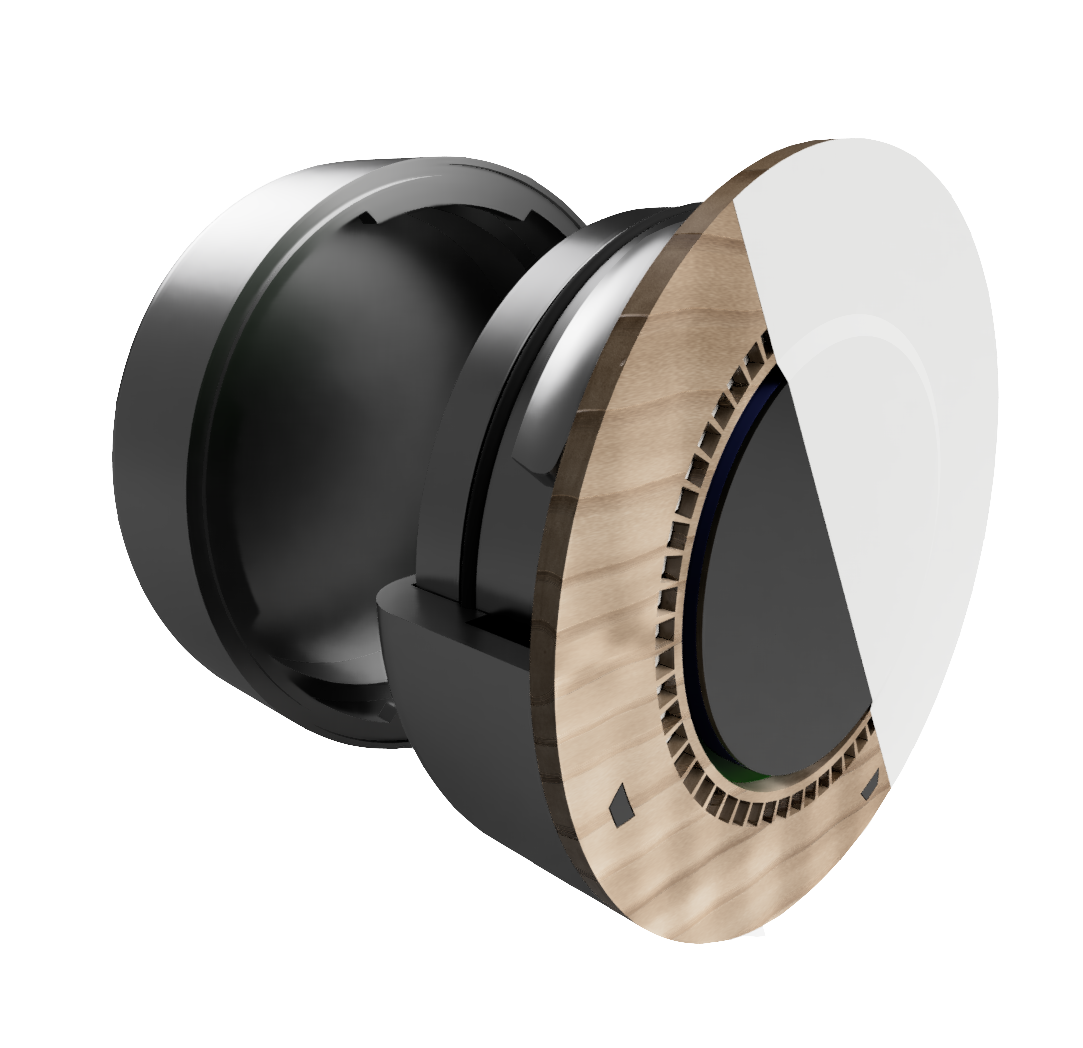
\includegraphics[width=0.15\textwidth]{kapitoly/obrazky/E4/B.B_Minibox.png}
    % }
    % \end{wrapfigure}
    \B{Mechanický BlackBox}
}

\fancyhead[LE,RO]{
    \B{příloha k~práci BlackBox}
}
\fancyfoot[CE,CO]{\leftmark}
\fancyfoot[LE,RO]{\thepage}

\renewcommand{\headrulewidth}{ 2pt } 
\renewcommand{\footrulewidth}{ 1pt }

\begin{document}

\maketitle

\pagestyle{empty}

\section*{Anotace}
\color{black}

Robotika se stává čím dál tím významnějším oborem, což s~sebou nese i~potřebu vzdělávání v~tomto oboru.
Pro naprosté začátečníky nebo lidi, kteří se nechtějí robotikou zabývat dlouhé stovky hodin, však nejsou vhodné 
relativně dražší elektronické stavebnice. Jedna z~nich je například elektronická varianta BlackBoxu, který má ohromné možnosti, 
ale to s~sebou pochopitelně nese i~potřebu jistých znalostí a~zkušeností.
Z~těchto důvodu jsem ze pustil i~do vývoje BlackBoxu v~čistě mechanické verzi.

\subsection*{Klíčová slova}

\color{black}

trezor, BlackBox, jednoduchá stavebnice, mechanická konstrukce % snadná robotika?

\newpage

\newpage

\tableofcontents % vysází obsah

\voffset = -40pt
\headsep = 20mm

\newpage

%%% Začátek práce
\setcounter{figure}{0}
\setcounter{table}{0}

\pagestyle{fancy}

\chapter{Úvod}
\thispagestyle{fancy}
Tato práce rozšiřuje informace o zařízeních BlackBox, což jsou primárně elektronická zařízení určená pro 
výuku robotiky, programování a jako platforma pro návrh a realizaci zážitkových akcí a táborových her.

Tato práce se věnuje méně sofistikovaným verzím BlackBoxu, které nemají žádnou elektroniku 
a jejich schopnosti jsou omezené jen na schopnost uzamčení menších předmětů, pomocí mechanicky určeného hesla.

Cílem práce je rozvést informace o mechanických verzích BlackBoxu, popsat jejich vývoj a možnosti jejich užití, 
včetně již existující reálné aplikace.

\chapter{Vývoj mechanického trezoru}
\thispagestyle{fancy}
\label{M-vyvoj}

\section{První verze}
\label{M1-vyvoj}

\begin{wrapfigure}{R}[20mm]{0.4\textwidth}
    \centering
    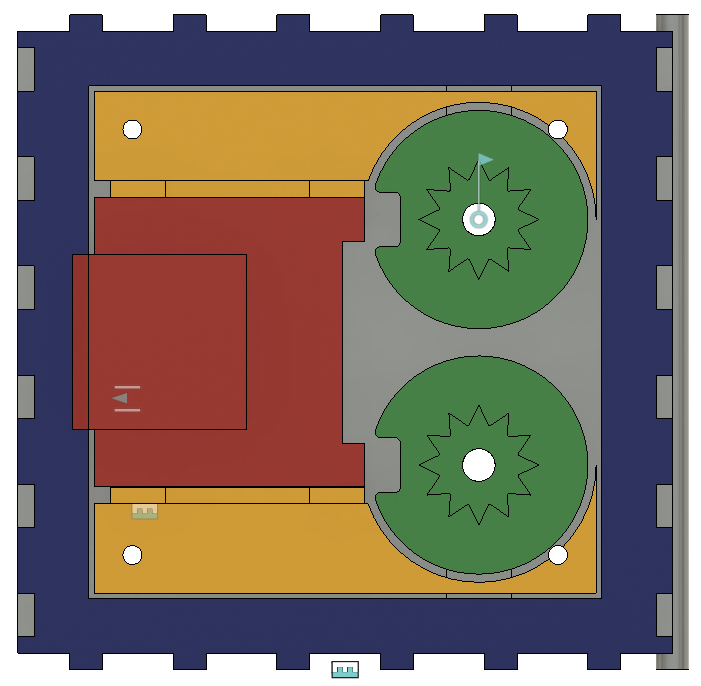
\includegraphics[width=0.4\textwidth]{kapitoly/obrazky/M1/mechanizmus.png}
    \caption{Zelená barva značí kódovací kola, červená západku, modrá pevnou část trezoru a žluté díly distanci \centering}
    \label{fig:M1-mechanizmus}
\end{wrapfigure}
První čistě mechanická varianta, označovaná jako M1, vznikla začátkem srpna 2019, brzy po první  elektronické variantě.
Měla stále poměrně klasický vzhled trezoru -- zamykatelná skříňka se dvěma  kódovacími koly, která ovládala možnost pohybu jednoduché západky.

Tato verze byla také určená jako základ pro plánovaný upgrade na další elektronickou
variantu. Na podobné vylepšení mělo stačit odstranění kódo\-va\-cích kol a přidělání elektronické části. Toto sice fungovalo obstojně, zároveň 
i~jako motivace, ale kvůli pozdější změně konceptu mechanizmu uzavírání trezoru\footnote{místo rotační západky mechanizmus bajonetu -- viz kapitola %todo
} tento nápad padl.

Tato varianta se také ukázala jako nevhodná\footnote{kvůli přílišné náročnosti na přesnost sesazení} pro stavbu s malými dětmi, 
pro které byla určena jakožto předstupeň k variantě elektronické (která vyžaduje i~znalosti programování nebo alespoň ochotu se jej  učit).

\newpage
\section{Druhá verze}

Druhá mechanická varianta má oproti první verzi daleko vetší počet možných kombinací.
Ovládá se pěti koly. Čtyři z nich nastavují heslo a páté otáčí s~rotační západkou, která drží dveře na svém místě.

Tato varianta taky přichází s možností dveře úplně oddělit od skříně trezoru. To by při využití jako trezor, který
má za úkol jen ochraňovat svůj obsah, sice nepřinášelo žádný velký užitek, ale při mém využití, spíše jako herní 
prvek než trezor, to může být užitečné.

\begin{figure}[htbp]
    \centering
    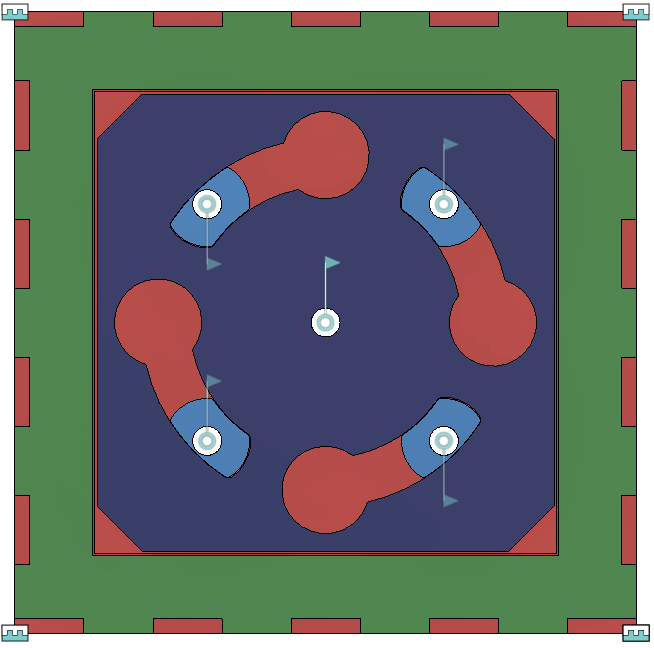
\includegraphics[width=150pt]{kapitoly/obrazky/M2/mechanizmus_odemcen.png}
    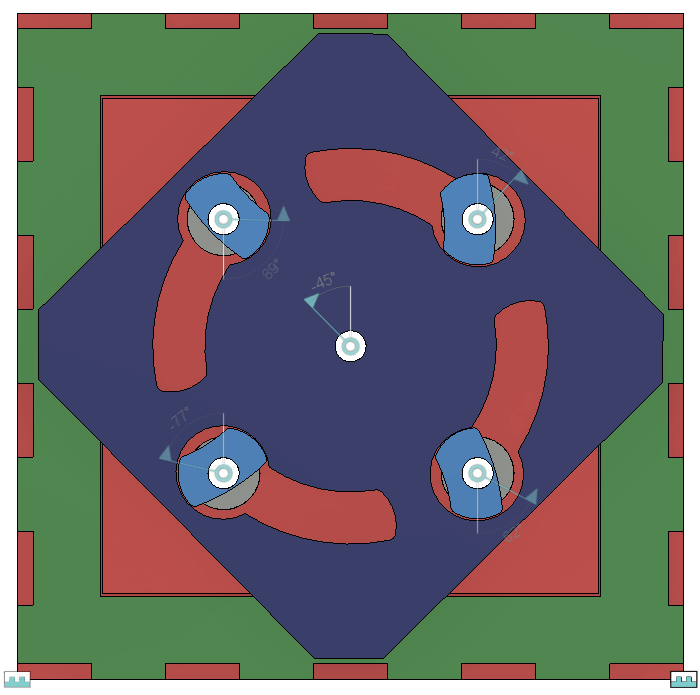
\includegraphics[width=150pt]{kapitoly/obrazky/M2/mechanizmus_zamceno.png}
    \caption{zamykací mechanizmus varianty M2}
    \label{fig:M2-mechanizmus}
\end{figure}

\begin{figure}[htbp]
    \centering
    \includegraphics[width=\textwidth]{kapitoly/obrazky/M2/predni_render.PNG}
    \caption{render varianty M2}
    \label{fig:M1.0}
\end{figure}


\newpage
\section{Třetí verze}

\begin{figure}[htbp]
    \centering
    \includegraphics[width=70pt]{kapitoly/obrazky/M3/predni_render.png}
    \caption{Render varianty M3}
    \label{fig:M3-render}
\end{figure}

Dnešní mechanická varianta je téměř stejná jako druhá verze, rozdíl je jen v~uložení kol, které kolem hřídelů získalo distanční kroužky, které
zjednodušují lepení. 

\begin{figure}[h]
    \centering
    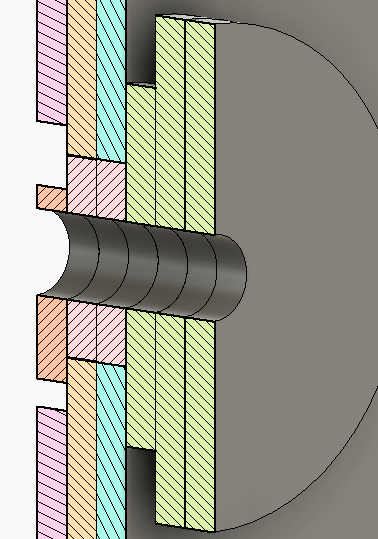
\includegraphics[width=0.4\textwidth]{kapitoly/obrazky/M3/rez.png}
    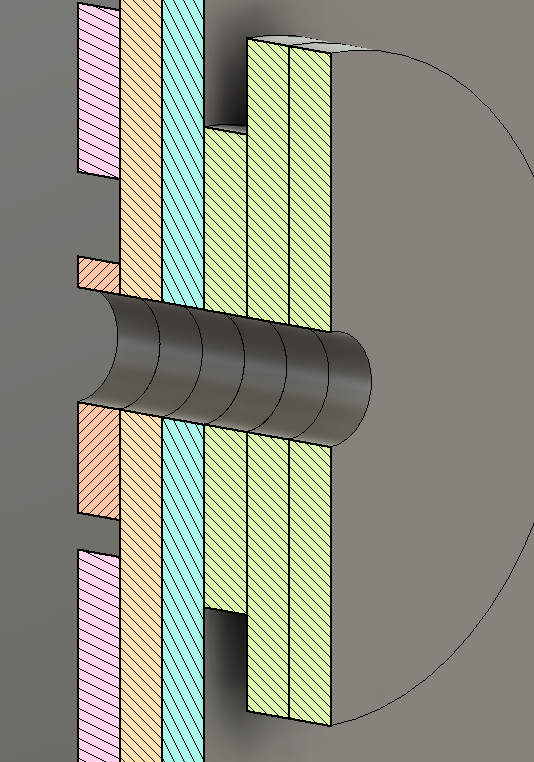
\includegraphics[width=0.4\textwidth]{kapitoly/obrazky/M2/rez.png}
    \caption{Řez kódovacím kolem trezoru M2 vlevo a řez kódovacím kolem trezoru M3 vpravo \centering}
    \label{fig:M3-rez-kolem}
\end{figure}

\newpage

\chapter{Mechanický trezor} 
\thispagestyle{fancy}
\label{M3}

\label{M3}
Vedle elektronické varianty jsem navrhl i~variantu čistě mechanickou, abych měl jednodušší 
a~levnější trezor pro mladší účastníky táborů a~jiných akcí. 
Mechanická varianta měla opět několik vývojových verzí. Jednotlivé verze a~jejich vlastnosti 
jsou popsány v~samostatné příloze. V~přílohách jsou také přiloženy výkresy poslední mechanické verze. 
Pro představu je v~příloze tohoto souboru uveden obrázek poslední mechanické verze \ref{fig:M2-render}. 

\begin{figure}[h]
	\centering
    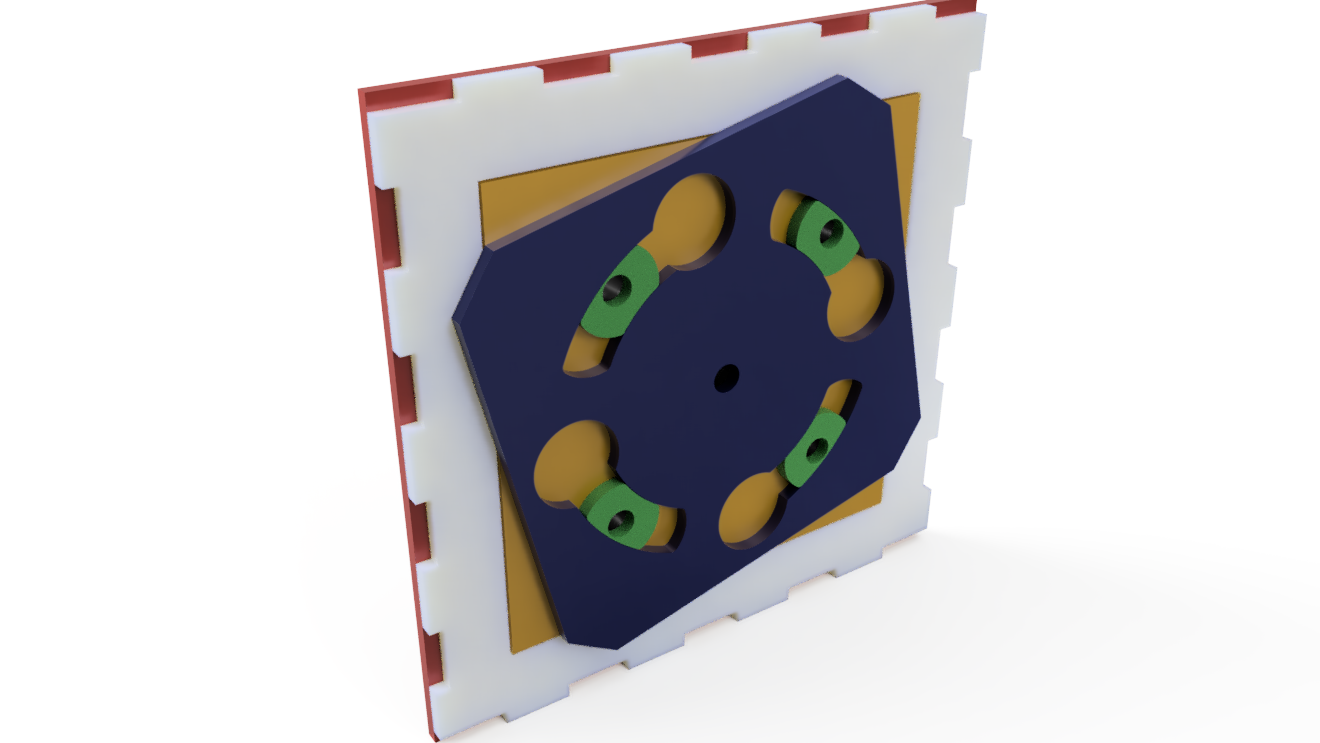
\includegraphics[width=\textwidth]{kapitoly/obrazky/M3/SOC_render.png}
    \caption{Vzhled mechanizmu zamykání u~mechanické verze}
    \label{fig:M3}
\end{figure}

\section{Popis jednotlivých součástek a důvody konkrétního tvaru}

\begin{wrapfigure}{R}[0.2\textwidth]{0.7\textwidth}
    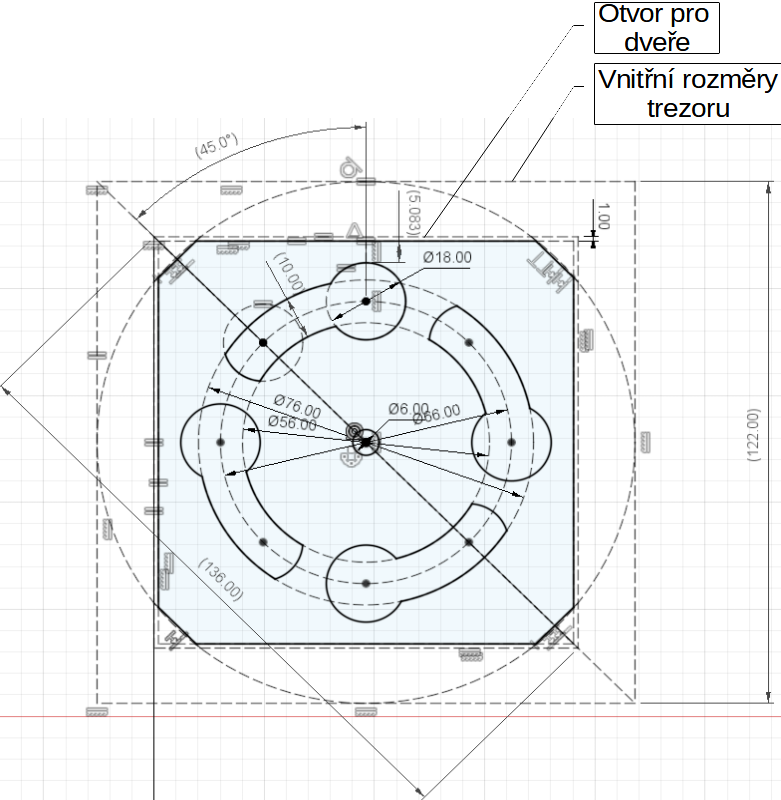
\includegraphics[width=0.7\textwidth]{kapitoly/obrazky/M3/geometrie_zapadky.png}
    \caption{náčrt} %todo čeho náčrt? 
    \label{fig:M3-geometrie-zapadky}
\end{wrapfigure} %todo zvážil bych obrázek centrovaný a obtékaný pouze nahoře a dole 

\subsection*{Geometrie západky}
Trezor má tvar krychle a~délku hrany má 128~mm, násobek šestnácti jsem zvolil kvůli jednoduché návaznosti na dřívka, %todo přidáme pár vět o dřívkách 
 dřevěná dřívka s obdélníkovým průřezem 3x16~mm nebo 2x16~mm. 
Protože je trezor vyroben z překližky o síle 4~mm, jsou jeho vnitřní rozměry o 4~mm na každé straně menší (takže 122~mm). 

%todo tady asi chybí další tvary? 
\section{Odolnost proti násilnému vniknutí}
Základní druhý namáhání, kterým musí trezor odolat, jsou

\begin{itemize}
    \item snaha o vytržení dveří 
    \item snaha o odemčení bez znalosti hesla
\end{itemize}

\paragraph{Vytržení dveří}
Jedním ze způsobů~namáhání~mechanizmu~je~vytržení~dveří~z~trezoru.

\subsection{Západka}

\begin{figure}[htbp]
    \centering
    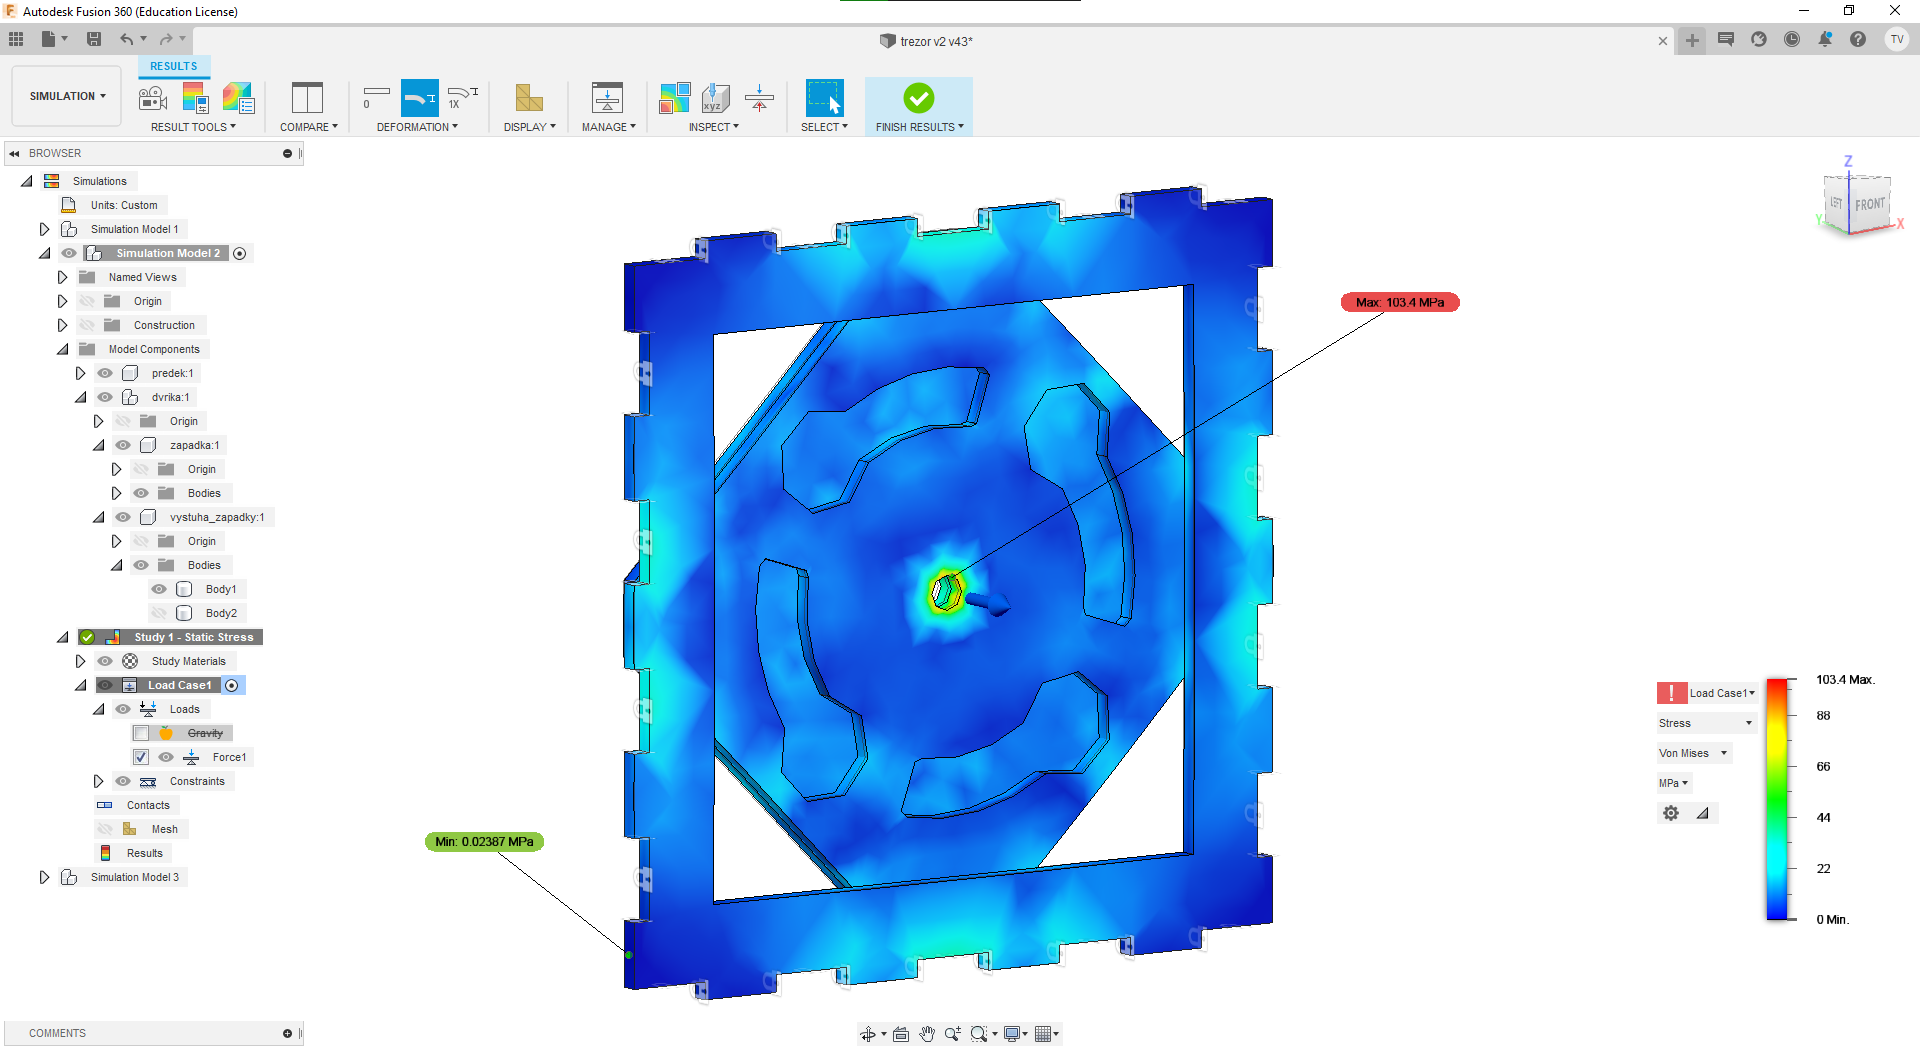
\includegraphics[width=\textwidth]{kapitoly/obrazky/M3/simulace/odolnost_proti_vytrzeni_4kN.png}
    \caption{Simulace pokusu o vytržení dveří silou 4 000 N}
    \label{fig:M3-simulace-vytrzeni}
\end{figure}
Ke kompletní simulaci se můžete dostat \href{https://myhub.autodesk360.com/ue2d7aa41/g/shares/SH56a43QTfd62c1cd96843f1e03a0eb48053?viewState=NoIgbgDAdAjCA0IDeAdEAXAngBwKZoC40BlASwFsBXAGwEN1SB7AOzXjVoGdPd1C0ARjABsATlEQItALQBjcbmkAWCMIjSBuWgA5lAM22ilAVgAmMAOyy9\%2BBGkYCAVrlnoAkqcIBmAL4gAukA}{zde}
po kliknutí na \uv{Simulation} a~\uv{Simulation Model 2}. V tabulce napravo se pak můžete přepínat mezi barevným zobrazení několika veličin.

\newpage

\subsection{Kolík}
Při pokusu o vytržení je celá síla přenášena kolíkem.

\begin{table}[h]
    \centering
    \resizebox{0.4\textwidth}{!}{%
    \begin{tabular}{l|l}
    $ \sigma $  & napětí v materiálu    \\
    $ D $       & průměr kolíku         \\
    $ F $       & působící síla         \\
    $ S $       & plocha průřezu kolíku \\
    \end{tabular}%
    }
    \caption{Tabulka použitých symbolu pro napětí v kolíku v tahu}
    \label{tab:M3_symboly_kolik}
\end{table}

 $ \sigma $     

 $ \sigma_{max} = 132  $ MPa    ( \href{https://is.mendelu.cz/eknihovna/opory/zobraz_cast.pl?fit_w=1;cast=9190}{dubové dřevo ve směru vláken při vlhkosti 12 \% }) % strana 22 tabulka 2 -> https://www.vutbr.cz/www_base/zav_prace_soubor_verejne.php?file_id=66237

$D = 6$ mm %todo popis všech veličin

 \(\sigma_{max} = F/S \Rightarrow F = \sigma_{max} \cdot S = 132 \cdot (\pi \cdot D^2/4) = 3 732,21 \) N  z toho a ze simulace vyplývá že kolík je při namáhání nejslabším členem.

\paragraph{Otevření bez odemčení}
Dalším způsobem namáhání může být snaha otočit západkou pez zadání správného hesla.

\subparagraph{Západka}

\begin{figure}[htbp]
    \centering
    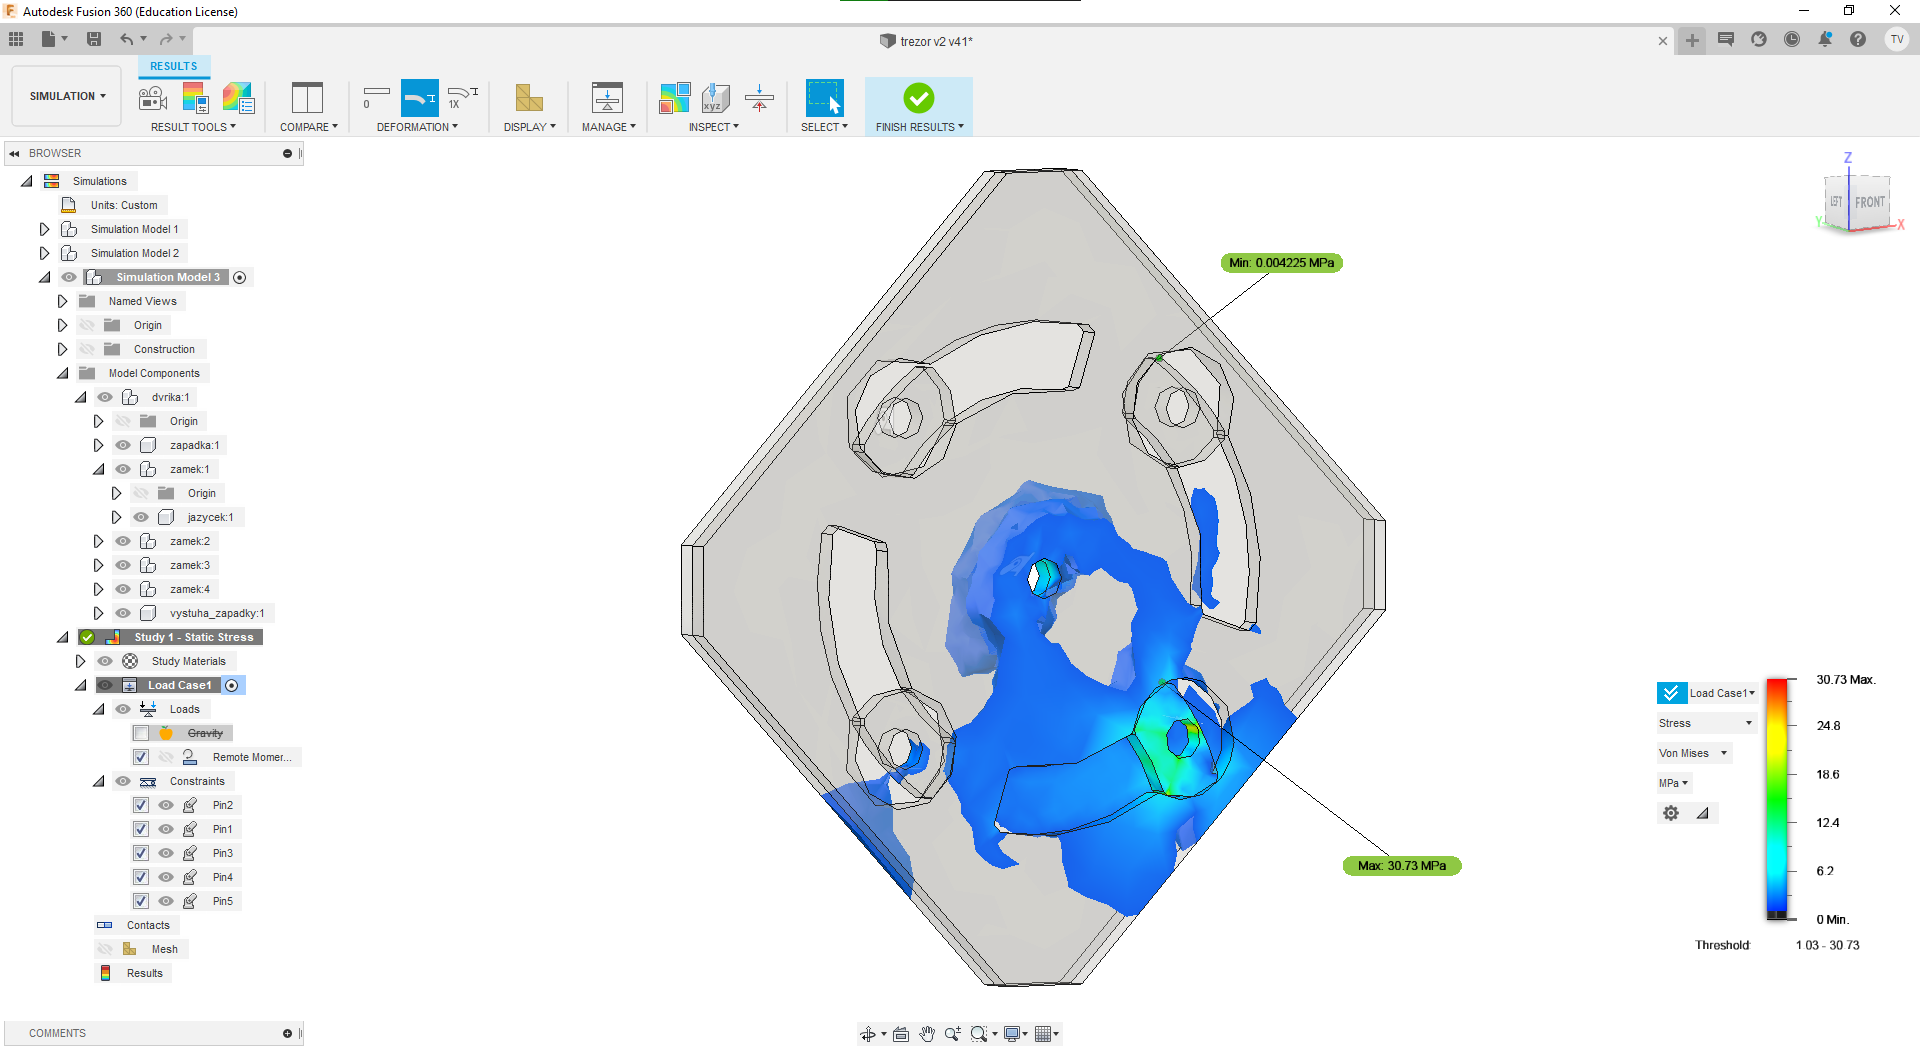
\includegraphics[width=\textwidth]{kapitoly/obrazky/M3/simulace/odolnost_proti_nasilnemu_odemceni_10Nm.png}
    \caption{Simulace pokusu o otevření bez předchozího odemčení při kroutícím momentu 10 000 Nmm, zobrazeno jen napětí nad 1 MPa}
    \label{fig:M3-simulace-vytrzeni}
\end{figure}

Ke kompletní simulaci se můžete dostat \href{https://myhub.autodesk360.com/ue2d7aa41/g/shares/SH56a43QTfd62c1cd96843f1e03a0eb48053?viewState=NoIgbgDAdAjCA0IDeAdEAXAngBwKZoC40BlASwFsBXAGwEN1SB7AOzXjVoGdPd1C0ARjABsATlEQItALQBjcbmkAWCMIjSBuWgA5lAM22ilAVgAmMAOyy9\%2BBGkYCAVrlnoAkqcIBmAL4gAukA}{zde}
po kliknutí na \uv{Simulation} a~\uv{Simulation Model 3}. V tabulce napravo se pak můžete přepínat mezi barevným zobrazení několika veličin.

\subparagraph{Kolík}
Kroutící moment, který je dřevěný kolík o průměru D = 6~mm schopen přenést. 

\begin{table}[h]
    \centering
    \resizebox{0.4\textwidth}{!}{%
    \begin{tabular}{l|l}
    $ \tau $    & napětí v materiálu při krutu      \\
    $ D    $    & průměr kolíku                     \\
    $ M_k  $    & kroutící moment                   \\
    $ W_k  $    & průřezový modul v krutu           \\
    \end{tabular}%
    }
    \caption{Tabulka použitých symbolu pro napětí v kolíku v tahu}
    \label{tab:M3_symboly_kolik}
\end{table}

$ \tau_{max} = 52,3 $ MPa (\href{https://is.mendelu.cz/eknihovna/opory/zobraz_cast.pl?fit_w=1;cast=9190}{dubové dřevo ve směru vláken při vlhkosti 12 \% })

$ \tau_{max} = \frac{M_k}{W_k} \Rightarrow M_k = \tau_{max} \cdot W_k = \tau _d \cdot \frac{\pi \cdot D^3}{16} $

$ M_k = 52,3 \cdot \frac{\pi \cdot 6^3}{16} = 2 218,16 $ N*mm. Z výpočtu a ze simulace plyne, že kolík je při namáhání v krutu nejslabším místem. Pro zvýšení odolnosti by proto bylo 
potřeba zvětšit kolík nebo změnit materiál.


\chapter{Závěr}
\thispagestyle{fancy}
Cílem této části mé práce bylo vyvinout čistě mechanický BlackBox pro mechanické stavby a~náplň různých 
kolektivních her. 
Cíle jsem dosáhl, zařízení je vyrobeno z překližky a dá se jednoduše sestavit za několik desítek minut. 

%todo   Seznam použitých odborných výrazů
%to-do      uvádí se významné odborné termíny s vysvětlením 
\newpage
\pagestyle{empty}
\pagestyle{plain}

\appendix
\phantomsection

\newcommand{\OdsazeniNadpisu}{10mm}
%\section{Vzhled druhé elektronické varianty} 
\begin{figure}

	
    %\vspace{\OdsazeniNadpisu}
    %\centering
    %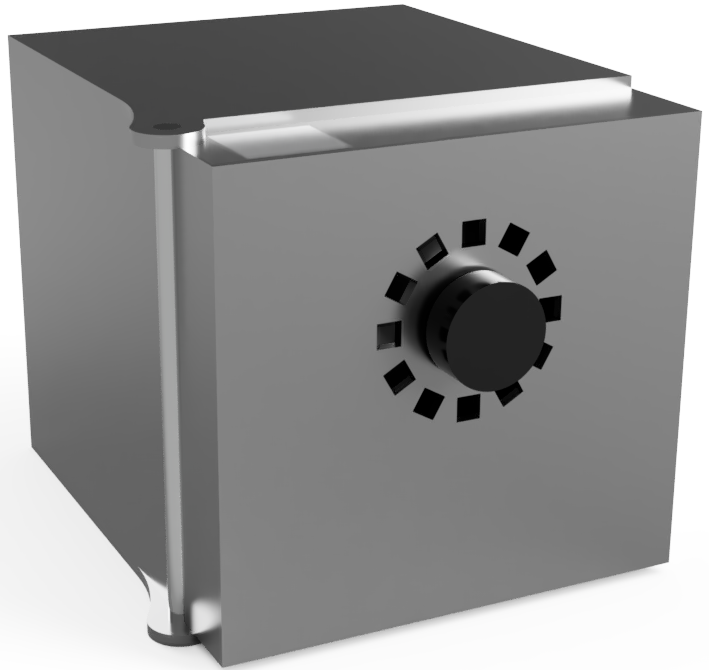
\includegraphics[width=0.5\textwidth]{kapitoly/obrazky/E2/predni_render.png}

    %\appendix
    \chapter{Obrazová příloha}
    \section{Vzhled první mechanické varianty}
	\centering
	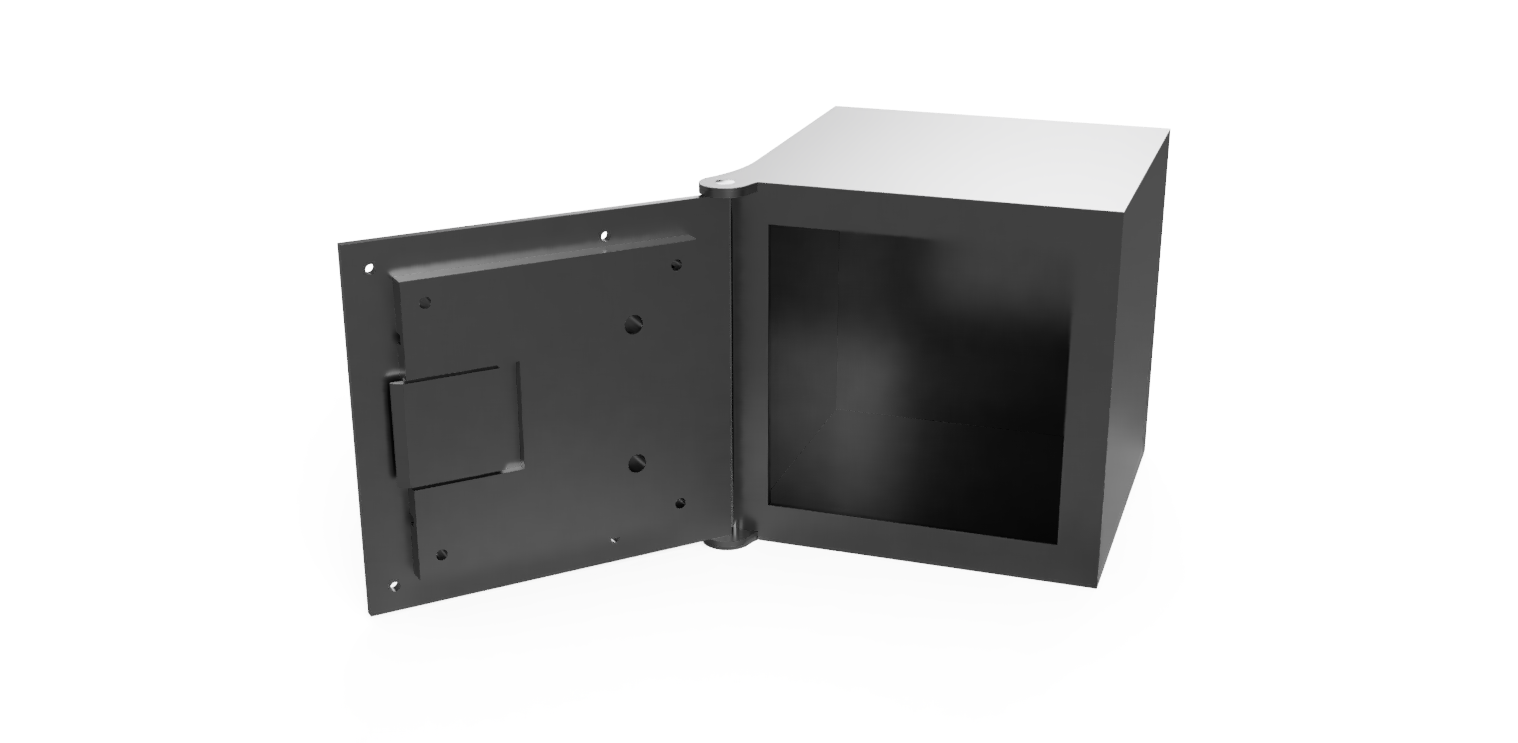
\includegraphics[width=\textwidth]{kapitoly/obrazky/M1/render.png}
	\caption{Render varianty M1}
	\label{fig:E3-renderi}
\end{figure}

\begin{figure}
    \section{Vzhled druhé elektronické varianty}
	\centering
	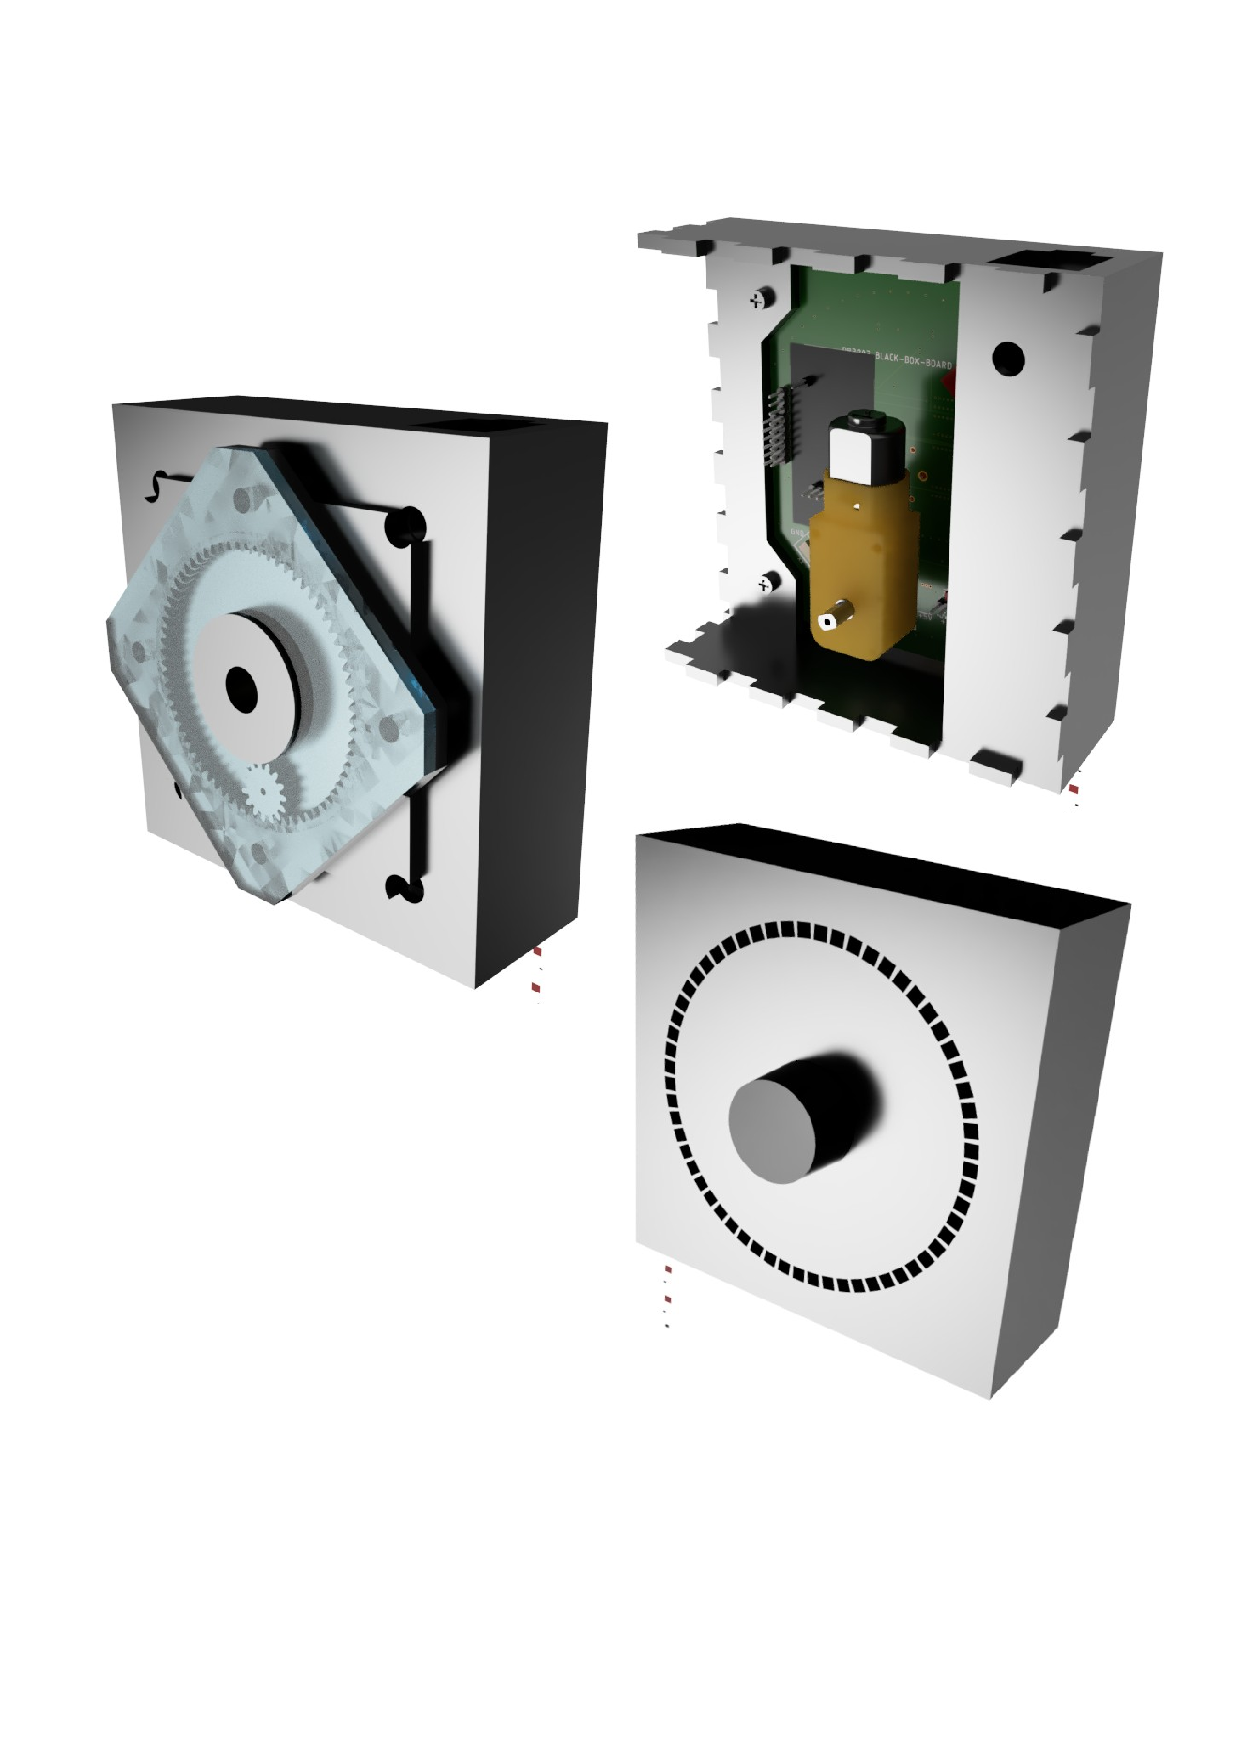
\includegraphics[width=\textwidth]{kapitoly/obrazky/E3/rendery.pdf}
	\caption{Render varianty M2}
	\label{fig:E3-renderi}
\end{figure}

\begin{figure}
	\section{Vzhled poslední mechanické varianty}
	\vspace{\OdsazeniNadpisu}
    \centering
    \includegraphics[width=\textwidth]{kapitoly/obrazky/M2/predni_render.PNG}
    \caption{Render varianty M3}
    \label{fig:M2-render}
\end{figure}


\phantomsection
\begin{figure}
    \chapter{Ostatní přílohy}
    \vspace{-30mm}
    \small
    \addtocounter{section}{1}
    \addcontentsline{toc}{section}{\protect\numberline{\thesection}Seznam obrázků} 
    \listoffigures
\end{figure}

% \phantomsection
% \normalsize
% \addtocounter{section}{1}
% \addcontentsline{toc}{section}{\protect\numberline{\thesection}Seznam tabulek}
% \listoftables

\phantomsection
\addtocounter{section}{1}
\addcontentsline{toc}{section}{\protect\numberline{\thesection}Literatura}
%\printbibheading
\printbibliography[title={Literatura}]

\end{document}